% Created:  Thu 10 Jul 2014 04:22 PM
% Modified: Wed 23 Jul 2014 05:30 PM
% @author Josh Wainwright
% File name : quadtree-traversal.tex

\section{Quadtree Traversal}
\label{sec:quadtree_traversal}

Whether the quadtree is stored in memory as a recursive quadtree data
structure, or as hash table, Section~\ref{sub:hash_table_implementation}, the
most important and computationally intensive step is extracting the clusters at
the correct depth and disregarding those data points that can be attributed to
noise.

The quadtree numbering system chosen lends itself very well to analysis based
on spatial location and the proximity of neighbours to a given node being
examined.

\subsection{Algorithm Description}
\label{sub:algorithm_description}

The propagation algorithm is performed as follows:
\begin{enumerate}
	\item Choose a starting location that has not yet been checked.
	\item For this given starting location, the $n$ neighbours are checked for
		validity based on the conditions of the analysis (the way these
		neighbours are selected is discussed in
		Section~\ref{sub:choosing_neighbours}).
	\item If a node fails the check, then it is recorded as having done so and
		shall not be checked again. If it passes, then it is itself propagated.
		\begin{itemize}
			\item To be ``propagated'' means the perform this propagation
				algorithm using that node as the starting location.
		\end{itemize}
	\item When all nodes have been checked, return to step 1.
	\item The algorithm completes either when either;
	\begin{itemize}
		\item every one of the nodes in the image have been checked and
			included or ignored, or
		\item the cluster has ended, so all the neighbours of all checked nodes
			have failed the validity tests and no further starting locations
			were found or specified.
	\end{itemize}
\end{enumerate}

This process is shown graphically in Figure~\ref{fig:propogation}. Here, and
from now on, blue nodes are nodes that either need to be checked or are
currently being checked; red are nodes that have been checked and have been
included in the cluster; question marks ({\footnotesize?}) represent the
neighbours of the blue nodes that will have to be checked to determine if it is
included or not and crosses ({\footnotesize x}) represent neighbours that have
been checked and excluded.

\begin{figure}[tbhp]
	\centering
	\includegraphics[width=0.88\linewidth]{propogation.pdf}
	\caption{For a starting location, a), in an image, no information is known
	and so the neighbours are checked. Some of these are found to be part of
	the cluster, others are rejected. The ones that are included are then,
	themselves, checked and so on. As the cluster grows, b), c) and d), the
	number of checked nodes increases.}
	\label{fig:propogation}
\end{figure}

When discovering clusters via this propagation technique, care must be taken to
avoid a run-away situation where every node in the tree gets included. This
would happen when looking at the neighbours of a node and blindly including
them. Since every internal node has exactly four neighbours, the propagation
would terminate only when reaching the edge nodes.

Instead, the depth of the node must be considered. Again, the simplest method
is not sufficient. If the propagation is limited to a given node depth, even if
this is not the same as the deepest node, the size of any clusters that are
identified will be limited, as shown in Figure~\ref{fig:propogation-halting}.
Since the depth to consider is not able to change, when the neighbours of the
blue node are checked, no correct neighbours are found and so the process
terminates. When able to view the larger structure of the nodes, however, it is
clear that the structure continues beyond the gap.

% \begin{figure}[tbhp]
% 	\centering
% 	\includegraphics[width=0.7\linewidth]{propogation-halting.pdf}
% 	% TODO caption
% 	\caption{propogation-Halting}
% 	\label{fig:propogation-halting}
% \end{figure}

% \begin{figure}[tbhp]
% 	\centering
% 	\includegraphics[width=0.88\linewidth]{propogation-levels.pdf}
% 	% TODO caption
% 	\caption{propogation-Levels}
% 	\label{fig:propogation-levels}
% \end{figure}

\begin{figure}[ht]
	\centering
	\begin{subfigure}[c]{0.6\linewidth}
		\includegraphics[width=\linewidth]{propogation-halting.pdf}
		\caption{} \label{fig:propogation-halting}
	\end{subfigure}%
	\quad
	\begin{subfigure}[c]{0.35\linewidth}
		\includegraphics[width=\linewidth]{propogation-levels.pdf}
		\caption{} \label{fig:propogation-levels}
	\end{subfigure}
		% TODO caption
	\caption{}\label{fig:prop-levels-halting}
\end{figure}

To avoid this, a certain amount of leniency must be given when deciding what
constitutes a neighbour. Given an appropriate value, this would allow both of
the larger white cells in Figure~\ref{fig:propogation-halting} to be included.

The \emph{depth range} shall define the levels that are to be considered when
choosing neighbours with respect to a target depth. Since clusters are being
considered as areas of increased density of points, all cells with a depth
greater than the target depth shall be allowed, so the purple cells in
Figure~\ref{fig:propogation-halting} would be included when the target depth is
the same as the depth of the included red cells. A depth range of zero is
equivalent to the situation above where only cells of a given depth are
considered. A depth range of 1 would mean that the white square in
Figure~\ref{fig:propogation-levels}\,i) would be included but not in~ii),
whereas a depth range of three would include both and so on.

\subsection{Clustering Start Locations}
\label{sub:clustering_start_locations}

In order for the algorithm to proceed correctly, a good initial node, a
starting location, must be chosen. Since the clusters to be found are regions
of high point density, it makes sense to start the clustering algorithm at the
point in the image with the highest point density. This should ensure that the
most defined cluster is always found with subsequent clusters being less dense,
and so less well defined.

When starting at the highest density node, i.e., the node which is at the
deepest level in the tree, propagating this node and then terminating; the
cluster shown in Figure~\ref{fig:single-cluster} is detected. The file
\texttt{palm-1.txt} was used and generated this data in
\SI{457}{\milli\second}. This shows that the algorithm works correctly.
Altering the parameters that are used to generate the quadtree affects the size
of the nodes that are included in the cluster and the depth that is searched.

\begin{figure}[tbhp]
	\centering
	\begin{subfigure}[c]{0.48\linewidth}
		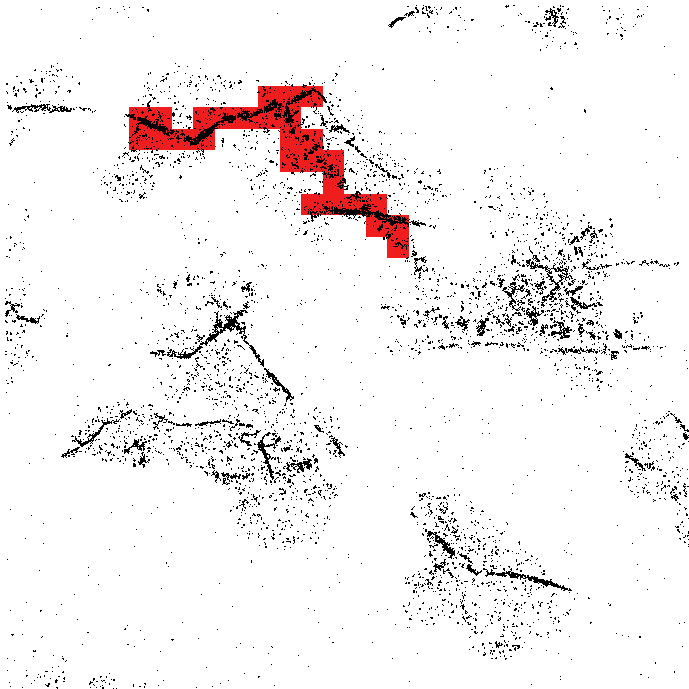
\includegraphics[width=\textwidth]{single-cluster.png}
		\caption{}\label{fig:single-cluster-points}
	\end{subfigure}%
	\quad
	\begin{subfigure}[c]{0.48\linewidth}
		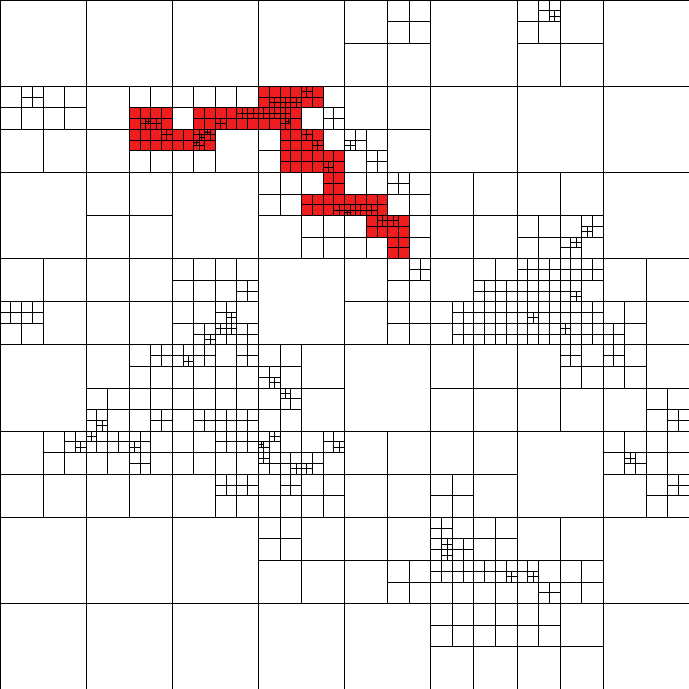
\includegraphics[width=\textwidth]{single-cluster-lines.png}
		\caption{}\label{fig:single-cluster-lines}
	\end{subfigure}
	% TODO caption
	\caption{single-cluster} \label{fig:single-cluster}
\end{figure}

\begin{figure}[tbhp]
	\begin{minipage}[c]{0.80\linewidth}
		\centering
		\fbox{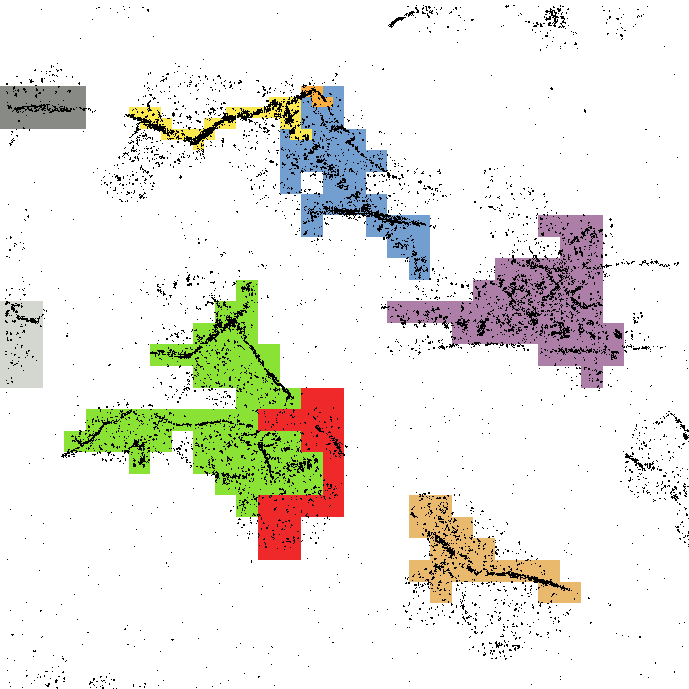
\includegraphics[width=\textwidth]{multiple-clusters-colours.png}}
	\end{minipage}%
	\quad
	\begin{minipage}[c]{0.1\linewidth}
		\centering
		\begin{tabular}[b]{ l l }
			\cellcolor[HTML]{FCE94F}1\\
			\cellcolor[HTML]{FCAF3E}2\\
			\cellcolor[HTML]{E9B96E}3\\
			\cellcolor[HTML]{8AE234}4\\
			\cellcolor[HTML]{729FCF}5\\
			\cellcolor[HTML]{AD7FA8}6\\
			\cellcolor[HTML]{EF2929}7\\
			\cellcolor[HTML]{D3D7CF}8\\
			\cellcolor[HTML]{888A85}9\\
		\end{tabular}
	\end{minipage}
	% TODO caption
	\caption{Bla bla}
	\label{fig:multiple-clusters-colours.png}
\end{figure}

\subsection{Choosing Neighbours}
\label{sub:choosing_neighbours}

Some care must be taken when deciding what constitutes a neighbour of a node
and what does not. As mentioned above, when detecting clusters using
propagation, the neighbours of a node are checked and, if they are valid, are
themselves propagated. For this reason, a poor choice of neighbours means that
either the propagation will
\begin{itemize}
	\item be cut short too early, and so not all of the clusters will be
		located, or
	\item include too many nodes, in which case the clusters will not represent
		the actual data.
\end{itemize}

The first neighbours that must be considered, named \emph{rook's case}
neighbours by~\cite{abel1990comparative}, are the four nodes that lie to the
north, east, sound and west of the current node. These are the nodes that are
directly in contact with the node and so, if they are valid, represent a direct
continuation of the cluster.

However, if the choice of neighbours is limited to these four, some major
structures are missed. Figure~\ref{fig:kernel-rooks-case} shows how this
arrangement misses a large portion of the cluster, simply because the
propagation could not consider the nodes across the boundary. If, in addition
to the rook's case, the four \emph{diagonal} neighbours are included, giving a
total of eight, the results are much better.

\begin{figure}[ht]
    \centering
    \begin{subfigure}[b]{0.48\linewidth}
        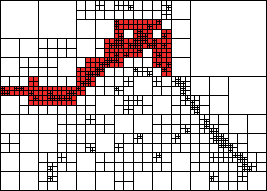
\includegraphics[width=\textwidth]{clusters/kernel-rooks-case.png}
        \caption{}\label{fig:kernel-rooks-case.png}
    \end{subfigure}%
    \quad
    \begin{subfigure}[b]{0.48\linewidth}
        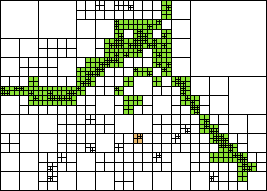
\includegraphics[width=\textwidth]{clusters/kernel-all8.png}
        \caption{}\label{fig:kernel-all8.png}
    \end{subfigure}
    % TODO caption
    \caption{}\label{fig:kernel-options}
\end{figure}
